% Options for packages loaded elsewhere
\PassOptionsToPackage{unicode}{hyperref}
\PassOptionsToPackage{hyphens}{url}
\PassOptionsToPackage{dvipsnames,svgnames,x11names}{xcolor}
%
\documentclass[
  letterpaper,
  DIV=11,
  numbers=noendperiod]{scrartcl}

\usepackage{amsmath,amssymb}
\usepackage{iftex}
\ifPDFTeX
  \usepackage[T1]{fontenc}
  \usepackage[utf8]{inputenc}
  \usepackage{textcomp} % provide euro and other symbols
\else % if luatex or xetex
  \usepackage{unicode-math}
  \defaultfontfeatures{Scale=MatchLowercase}
  \defaultfontfeatures[\rmfamily]{Ligatures=TeX,Scale=1}
\fi
\usepackage{lmodern}
\ifPDFTeX\else  
    % xetex/luatex font selection
\fi
% Use upquote if available, for straight quotes in verbatim environments
\IfFileExists{upquote.sty}{\usepackage{upquote}}{}
\IfFileExists{microtype.sty}{% use microtype if available
  \usepackage[]{microtype}
  \UseMicrotypeSet[protrusion]{basicmath} % disable protrusion for tt fonts
}{}
\makeatletter
\@ifundefined{KOMAClassName}{% if non-KOMA class
  \IfFileExists{parskip.sty}{%
    \usepackage{parskip}
  }{% else
    \setlength{\parindent}{0pt}
    \setlength{\parskip}{6pt plus 2pt minus 1pt}}
}{% if KOMA class
  \KOMAoptions{parskip=half}}
\makeatother
\usepackage{xcolor}
\setlength{\emergencystretch}{3em} % prevent overfull lines
\setcounter{secnumdepth}{-\maxdimen} % remove section numbering
% Make \paragraph and \subparagraph free-standing
\makeatletter
\ifx\paragraph\undefined\else
  \let\oldparagraph\paragraph
  \renewcommand{\paragraph}{
    \@ifstar
      \xxxParagraphStar
      \xxxParagraphNoStar
  }
  \newcommand{\xxxParagraphStar}[1]{\oldparagraph*{#1}\mbox{}}
  \newcommand{\xxxParagraphNoStar}[1]{\oldparagraph{#1}\mbox{}}
\fi
\ifx\subparagraph\undefined\else
  \let\oldsubparagraph\subparagraph
  \renewcommand{\subparagraph}{
    \@ifstar
      \xxxSubParagraphStar
      \xxxSubParagraphNoStar
  }
  \newcommand{\xxxSubParagraphStar}[1]{\oldsubparagraph*{#1}\mbox{}}
  \newcommand{\xxxSubParagraphNoStar}[1]{\oldsubparagraph{#1}\mbox{}}
\fi
\makeatother

\usepackage{color}
\usepackage{fancyvrb}
\newcommand{\VerbBar}{|}
\newcommand{\VERB}{\Verb[commandchars=\\\{\}]}
\DefineVerbatimEnvironment{Highlighting}{Verbatim}{commandchars=\\\{\}}
% Add ',fontsize=\small' for more characters per line
\usepackage{framed}
\definecolor{shadecolor}{RGB}{241,243,245}
\newenvironment{Shaded}{\begin{snugshade}}{\end{snugshade}}
\newcommand{\AlertTok}[1]{\textcolor[rgb]{0.68,0.00,0.00}{#1}}
\newcommand{\AnnotationTok}[1]{\textcolor[rgb]{0.37,0.37,0.37}{#1}}
\newcommand{\AttributeTok}[1]{\textcolor[rgb]{0.40,0.45,0.13}{#1}}
\newcommand{\BaseNTok}[1]{\textcolor[rgb]{0.68,0.00,0.00}{#1}}
\newcommand{\BuiltInTok}[1]{\textcolor[rgb]{0.00,0.23,0.31}{#1}}
\newcommand{\CharTok}[1]{\textcolor[rgb]{0.13,0.47,0.30}{#1}}
\newcommand{\CommentTok}[1]{\textcolor[rgb]{0.37,0.37,0.37}{#1}}
\newcommand{\CommentVarTok}[1]{\textcolor[rgb]{0.37,0.37,0.37}{\textit{#1}}}
\newcommand{\ConstantTok}[1]{\textcolor[rgb]{0.56,0.35,0.01}{#1}}
\newcommand{\ControlFlowTok}[1]{\textcolor[rgb]{0.00,0.23,0.31}{\textbf{#1}}}
\newcommand{\DataTypeTok}[1]{\textcolor[rgb]{0.68,0.00,0.00}{#1}}
\newcommand{\DecValTok}[1]{\textcolor[rgb]{0.68,0.00,0.00}{#1}}
\newcommand{\DocumentationTok}[1]{\textcolor[rgb]{0.37,0.37,0.37}{\textit{#1}}}
\newcommand{\ErrorTok}[1]{\textcolor[rgb]{0.68,0.00,0.00}{#1}}
\newcommand{\ExtensionTok}[1]{\textcolor[rgb]{0.00,0.23,0.31}{#1}}
\newcommand{\FloatTok}[1]{\textcolor[rgb]{0.68,0.00,0.00}{#1}}
\newcommand{\FunctionTok}[1]{\textcolor[rgb]{0.28,0.35,0.67}{#1}}
\newcommand{\ImportTok}[1]{\textcolor[rgb]{0.00,0.46,0.62}{#1}}
\newcommand{\InformationTok}[1]{\textcolor[rgb]{0.37,0.37,0.37}{#1}}
\newcommand{\KeywordTok}[1]{\textcolor[rgb]{0.00,0.23,0.31}{\textbf{#1}}}
\newcommand{\NormalTok}[1]{\textcolor[rgb]{0.00,0.23,0.31}{#1}}
\newcommand{\OperatorTok}[1]{\textcolor[rgb]{0.37,0.37,0.37}{#1}}
\newcommand{\OtherTok}[1]{\textcolor[rgb]{0.00,0.23,0.31}{#1}}
\newcommand{\PreprocessorTok}[1]{\textcolor[rgb]{0.68,0.00,0.00}{#1}}
\newcommand{\RegionMarkerTok}[1]{\textcolor[rgb]{0.00,0.23,0.31}{#1}}
\newcommand{\SpecialCharTok}[1]{\textcolor[rgb]{0.37,0.37,0.37}{#1}}
\newcommand{\SpecialStringTok}[1]{\textcolor[rgb]{0.13,0.47,0.30}{#1}}
\newcommand{\StringTok}[1]{\textcolor[rgb]{0.13,0.47,0.30}{#1}}
\newcommand{\VariableTok}[1]{\textcolor[rgb]{0.07,0.07,0.07}{#1}}
\newcommand{\VerbatimStringTok}[1]{\textcolor[rgb]{0.13,0.47,0.30}{#1}}
\newcommand{\WarningTok}[1]{\textcolor[rgb]{0.37,0.37,0.37}{\textit{#1}}}

\providecommand{\tightlist}{%
  \setlength{\itemsep}{0pt}\setlength{\parskip}{0pt}}\usepackage{longtable,booktabs,array}
\usepackage{calc} % for calculating minipage widths
% Correct order of tables after \paragraph or \subparagraph
\usepackage{etoolbox}
\makeatletter
\patchcmd\longtable{\par}{\if@noskipsec\mbox{}\fi\par}{}{}
\makeatother
% Allow footnotes in longtable head/foot
\IfFileExists{footnotehyper.sty}{\usepackage{footnotehyper}}{\usepackage{footnote}}
\makesavenoteenv{longtable}
\usepackage{graphicx}
\makeatletter
\def\maxwidth{\ifdim\Gin@nat@width>\linewidth\linewidth\else\Gin@nat@width\fi}
\def\maxheight{\ifdim\Gin@nat@height>\textheight\textheight\else\Gin@nat@height\fi}
\makeatother
% Scale images if necessary, so that they will not overflow the page
% margins by default, and it is still possible to overwrite the defaults
% using explicit options in \includegraphics[width, height, ...]{}
\setkeys{Gin}{width=\maxwidth,height=\maxheight,keepaspectratio}
% Set default figure placement to htbp
\makeatletter
\def\fps@figure{htbp}
\makeatother

\usepackage{fvextra}
\DefineVerbatimEnvironment{Highlighting}{Verbatim}{breaklines,commandchars=\\\{\}}
\KOMAoption{captions}{tableheading}
\makeatletter
\@ifpackageloaded{caption}{}{\usepackage{caption}}
\AtBeginDocument{%
\ifdefined\contentsname
  \renewcommand*\contentsname{Table of contents}
\else
  \newcommand\contentsname{Table of contents}
\fi
\ifdefined\listfigurename
  \renewcommand*\listfigurename{List of Figures}
\else
  \newcommand\listfigurename{List of Figures}
\fi
\ifdefined\listtablename
  \renewcommand*\listtablename{List of Tables}
\else
  \newcommand\listtablename{List of Tables}
\fi
\ifdefined\figurename
  \renewcommand*\figurename{Figure}
\else
  \newcommand\figurename{Figure}
\fi
\ifdefined\tablename
  \renewcommand*\tablename{Table}
\else
  \newcommand\tablename{Table}
\fi
}
\@ifpackageloaded{float}{}{\usepackage{float}}
\floatstyle{ruled}
\@ifundefined{c@chapter}{\newfloat{codelisting}{h}{lop}}{\newfloat{codelisting}{h}{lop}[chapter]}
\floatname{codelisting}{Listing}
\newcommand*\listoflistings{\listof{codelisting}{List of Listings}}
\makeatother
\makeatletter
\makeatother
\makeatletter
\@ifpackageloaded{caption}{}{\usepackage{caption}}
\@ifpackageloaded{subcaption}{}{\usepackage{subcaption}}
\makeatother

\ifLuaTeX
  \usepackage{selnolig}  % disable illegal ligatures
\fi
\usepackage{bookmark}

\IfFileExists{xurl.sty}{\usepackage{xurl}}{} % add URL line breaks if available
\urlstyle{same} % disable monospaced font for URLs
\hypersetup{
  pdftitle={PS4 Andy Fan Will Sigal},
  colorlinks=true,
  linkcolor={blue},
  filecolor={Maroon},
  citecolor={Blue},
  urlcolor={Blue},
  pdfcreator={LaTeX via pandoc}}


\title{PS4 Andy Fan Will Sigal}
\author{}
\date{}

\begin{document}
\maketitle

\RecustomVerbatimEnvironment{verbatim}{Verbatim}{
  showspaces = false,
  showtabs = false,
  breaksymbolleft={},
  breaklines
}


\textbf{PS4:} Due Sat Nov 2 at 5:00PM Central. Worth 100 points.

\subsection{Style Points (10 pts)}\label{style-points-10-pts}

\subsection{Submission Steps (10 pts)}\label{submission-steps-10-pts}

\begin{enumerate}
\def\labelenumi{\arabic{enumi}.}
\tightlist
\item
  This problem set is a paired problem set.
\item
  Play paper, scissors, rock to determine who goes first. Call that
  person \emph{Partner 1}.

  \begin{itemize}
  \tightlist
  \item
    Partner 1 (name and cnet ID): Andy Fan, fanx
  \item
    Partner 2 (name and cnet ID):
  \end{itemize}
\item
  Partner 1 will accept the \texttt{ps4} and then share the link it
  creates with their partner. You can only share it with one partner so
  you will not be able to change it after your partner has accepted.
\item
  ``This submission is our work alone and complies with the 30538
  integrity policy.'' Add your initials to indicate your agreement:
\end{enumerate}

AF WS

\begin{enumerate}
\def\labelenumi{\arabic{enumi}.}
\setcounter{enumi}{4}
\tightlist
\item
  ``I have uploaded the names of anyone else other than my partner and I
  worked with on the problem set
  \textbf{\href{https://docs.google.com/forms/d/185usrCREQaUbvAXpWhChkjghdGgmAZXA3lPWpXLLsts/edit}{here}}''
  (1 point)
\item
  Late coins used this pset: (Andy:0); (will:0) Late coins left after
  submission: (Andy: 3) ; (will: 4)
\item
  Knit your \texttt{ps4.qmd} to an PDF file to make \texttt{ps4.pdf},

  \begin{itemize}
  \tightlist
  \item
    The PDF should not be more than 25 pages. Use \texttt{head()} and
    re-size figures when appropriate.
  \end{itemize}
\item
  (Partner 1): push \texttt{ps4.qmd} and \texttt{ps4.pdf} to your github
  repo.
\item
  (Partner 1): submit \texttt{ps4.pdf} via Gradescope. Add your partner
  on Gradescope.
\item
  (Partner 1): tag your submission in Gradescope
\end{enumerate}

\textbf{Important:} Repositories are for tracking code. \textbf{Do not
commit the data or shapefiles to your repo.} The best way to do this is
with \texttt{.gitignore}, which we have covered in class. If you do
accidentally commit the data, Github has a
\href{https://docs.github.com/en/repositories/working-with-files/managing-large-files/about-large-files-on-github\#removing-files-from-a-repositorys-history}{guide}.
The best course of action depends on whether you have pushed yet. This
also means that both partners will have to download the initial raw data
and any data cleaning code will need to be re-run on both partners'
computers.

\subsection{Download and explore the Provider of Services (POS) file (10
pts)}\label{download-and-explore-the-provider-of-services-pos-file-10-pts}

(This file records all providers certified to bill Medicare and
Medicaid. Each provider has a unique CMS certification number,
consistent across different years)

(The data dictionary is located at the bottom of the page as ``Provider
of Services File- Hospital \& Non-Hospital Facilities Data Dictionary)

\begin{Shaded}
\begin{Highlighting}[]
\CommentTok{\#\#\# SETUP }
\ImportTok{import}\NormalTok{ pandas }\ImportTok{as}\NormalTok{ pd}
\ImportTok{import}\NormalTok{ altair }\ImportTok{as}\NormalTok{ alt}
\ImportTok{import}\NormalTok{ time}
\ImportTok{import}\NormalTok{ os}
\ImportTok{import}\NormalTok{ warnings }
\NormalTok{warnings.filterwarnings(}\StringTok{\textquotesingle{}ignore\textquotesingle{}}\NormalTok{)}
\end{Highlighting}
\end{Shaded}

\paragraph{1. (Partner 1) This is a fairly large dataset and we won't be
using most of the variables. Read through the rest of the problem set
and look through the data dictionary to identify which variables you
will need to complete the exercise, and use the tool on data.cms.gov
into restrict to those variables (``Manage Columns'') before exporting
(``Export''). Download this for 2016 and call it pos2016.csv. What are
the variables you
pulled?}\label{partner-1-this-is-a-fairly-large-dataset-and-we-wont-be-using-most-of-the-variables.-read-through-the-rest-of-the-problem-set-and-look-through-the-data-dictionary-to-identify-which-variables-you-will-need-to-complete-the-exercise-and-use-the-tool-on-data.cms.gov-into-restrict-to-those-variables-manage-columns-before-exporting-export.-download-this-for-2016-and-call-it-pos2016.csv.-what-are-the-variables-you-pulled}

required variables:

provider type code: PRVDR\_CTGRY\_CD

subtype code: PRVDR\_CTGRY\_SBTYP\_CD

CMS certification number: PRVDR\_NUM

Termination code: PGM\_TRMNTN\_CD

zip code: ZIP\_CD

Date of termination: TRMNTN\_EXPRTN\_DT

Facility name: FAC\_NAME

\begin{Shaded}
\begin{Highlighting}[]
\CommentTok{\#\#\# import data (default directory is just the repo)}

\CommentTok{\#os.chdir(\textquotesingle{}/Users/willsigal/Documents/GitHub/problem{-}set{-}4{-}andy{-}fan{-}will{-}sigal\textquotesingle{}) \#will wd}

\NormalTok{os.chdir(}\StringTok{\textquotesingle{}d:}\CharTok{\textbackslash{}\textbackslash{}}\StringTok{UChicago}\CharTok{\textbackslash{}\textbackslash{}}\StringTok{Classes}\CharTok{\textbackslash{}\textbackslash{}}\StringTok{2024Qfall}\CharTok{\textbackslash{}\textbackslash{}}\StringTok{Programming Python}\CharTok{\textbackslash{}\textbackslash{}}\StringTok{problem{-}set{-}4{-}andy{-}fan{-}will{-}sigal\textquotesingle{}}\NormalTok{) }\CommentTok{\#andy wd}

\NormalTok{df\_2016 }\OperatorTok{=}\NormalTok{ pd.read\_csv(}\StringTok{\textquotesingle{}pos2016.csv\textquotesingle{}}\NormalTok{, encoding}\OperatorTok{=}\StringTok{"latin1"}\NormalTok{, on\_bad\_lines}\OperatorTok{=}\StringTok{"skip"}\NormalTok{)}
\end{Highlighting}
\end{Shaded}

\paragraph{2. (Partner 1) Import your pos2016.csv file. We want to focus
on short-term hospitals. These are identified as facilities with
provider type code 01 and subtype code 01. Subset your data to these
facilities. How many hospitals are reported in this data? Does this
number make sense? Cross-reference with other sources and cite the
number you compared it to. If it differs, why do you think it could
differ?}\label{partner-1-import-your-pos2016.csv-file.-we-want-to-focus-on-short-term-hospitals.-these-are-identified-as-facilities-with-provider-type-code-01-and-subtype-code-01.-subset-your-data-to-these-facilities.-how-many-hospitals-are-reported-in-this-data-does-this-number-make-sense-cross-reference-with-other-sources-and-cite-the-number-you-compared-it-to.-if-it-differs-why-do-you-think-it-could-differ}

\begin{Shaded}
\begin{Highlighting}[]
\CommentTok{\#\#\#subset to short term hositals}
\NormalTok{df\_2016 }\OperatorTok{=}\NormalTok{ df\_2016[(df\_2016[}\StringTok{\textquotesingle{}PRVDR\_CTGRY\_SBTYP\_CD\textquotesingle{}}\NormalTok{] }\OperatorTok{==} \DecValTok{1}\NormalTok{) }\OperatorTok{\&}\NormalTok{ (df\_2016[}\StringTok{\textquotesingle{}PRVDR\_CTGRY\_CD\textquotesingle{}}\NormalTok{] }\OperatorTok{==} \DecValTok{1}\NormalTok{)]}
\end{Highlighting}
\end{Shaded}

\begin{verbatim}
a.There are 7275 short term hospitals reported in the data. This number at a glance makes sense nationwide.

b.Looking at the Article by Jane Wishner, Patricia Solleveld, Robin Rudowitz, Julia Paradise, and Larisa Antonisse, they found "nearly 5,000 short-term, acute care hospitals in the United States". This is less than the data we have. It is possibly because some of the short-term hospitals in our dataset closed (they are temporary after all, and could have only been setup for less than a year)
\end{verbatim}

\paragraph{3. (Partner 1) Repeat the previous 3 steps with 2017Q4,
2018Q4, and 2019Q4 and then append them together. Plot the number of
observations in your dataset by
year.}\label{partner-1-repeat-the-previous-3-steps-with-2017q4-2018q4-and-2019q4-and-then-append-them-together.-plot-the-number-of-observations-in-your-dataset-by-year.}

\begin{Shaded}
\begin{Highlighting}[]
\CommentTok{\#\#\# import data }
\NormalTok{df\_2017 }\OperatorTok{=}\NormalTok{ pd.read\_csv(}\StringTok{\textquotesingle{}pos2017.csv\textquotesingle{}}\NormalTok{, encoding}\OperatorTok{=}\StringTok{"latin1"}\NormalTok{, on\_bad\_lines}\OperatorTok{=}\StringTok{"skip"}\NormalTok{)}

\NormalTok{df\_2018 }\OperatorTok{=}\NormalTok{ pd.read\_csv(}\StringTok{\textquotesingle{}pos2018.csv\textquotesingle{}}\NormalTok{, encoding}\OperatorTok{=}\StringTok{"latin1"}\NormalTok{, on\_bad\_lines}\OperatorTok{=}\StringTok{"skip"}\NormalTok{)}

\NormalTok{df\_2019 }\OperatorTok{=}\NormalTok{ pd.read\_csv(}\StringTok{\textquotesingle{}pos2019.csv\textquotesingle{}}\NormalTok{, encoding}\OperatorTok{=}\StringTok{"latin1"}\NormalTok{, on\_bad\_lines}\OperatorTok{=}\StringTok{"skip"}\NormalTok{)}
\end{Highlighting}
\end{Shaded}

\begin{Shaded}
\begin{Highlighting}[]
\CommentTok{\#\#\#subset to short term hositals}
\NormalTok{df\_2017 }\OperatorTok{=}\NormalTok{ df\_2017[(df\_2017[}\StringTok{\textquotesingle{}PRVDR\_CTGRY\_SBTYP\_CD\textquotesingle{}}\NormalTok{] }\OperatorTok{==} \DecValTok{1}\NormalTok{) }\OperatorTok{\&}\NormalTok{ (df\_2017[}\StringTok{\textquotesingle{}PRVDR\_CTGRY\_CD\textquotesingle{}}\NormalTok{] }\OperatorTok{==} \DecValTok{1}\NormalTok{)]}
\NormalTok{df\_2018 }\OperatorTok{=}\NormalTok{ df\_2018[(df\_2018[}\StringTok{\textquotesingle{}PRVDR\_CTGRY\_SBTYP\_CD\textquotesingle{}}\NormalTok{] }\OperatorTok{==} \DecValTok{1}\NormalTok{) }\OperatorTok{\&}\NormalTok{ (df\_2018[}\StringTok{\textquotesingle{}PRVDR\_CTGRY\_CD\textquotesingle{}}\NormalTok{] }\OperatorTok{==} \DecValTok{1}\NormalTok{)]}
\NormalTok{df\_2019 }\OperatorTok{=}\NormalTok{ df\_2019[(df\_2019[}\StringTok{\textquotesingle{}PRVDR\_CTGRY\_SBTYP\_CD\textquotesingle{}}\NormalTok{] }\OperatorTok{==} \DecValTok{1}\NormalTok{) }\OperatorTok{\&}\NormalTok{ (df\_2019[}\StringTok{\textquotesingle{}PRVDR\_CTGRY\_CD\textquotesingle{}}\NormalTok{] }\OperatorTok{==} \DecValTok{1}\NormalTok{)]}
\end{Highlighting}
\end{Shaded}

The number of short-term hospitals in each of the years:

2017: 7260 hospitals

2018: 7277 hospitals

2019: 7303 hospitals

\begin{Shaded}
\begin{Highlighting}[]
\CommentTok{\#\#\# create new year columns}
\NormalTok{df\_2016[}\StringTok{\textquotesingle{}year\textquotesingle{}}\NormalTok{] }\OperatorTok{=} \DecValTok{2016}
\NormalTok{df\_2017[}\StringTok{\textquotesingle{}year\textquotesingle{}}\NormalTok{] }\OperatorTok{=} \DecValTok{2017}
\NormalTok{df\_2018[}\StringTok{\textquotesingle{}year\textquotesingle{}}\NormalTok{] }\OperatorTok{=} \DecValTok{2018}
\NormalTok{df\_2019[}\StringTok{\textquotesingle{}year\textquotesingle{}}\NormalTok{] }\OperatorTok{=} \DecValTok{2019}

\CommentTok{\#\#\# append}
\NormalTok{df }\OperatorTok{=}\NormalTok{ pd.concat([df\_2016, df\_2017, df\_2018, df\_2019], ignore\_index}\OperatorTok{=}\VariableTok{True}\NormalTok{)}
\end{Highlighting}
\end{Shaded}

\begin{Shaded}
\begin{Highlighting}[]
\CommentTok{\#\#\# altair plot}
\NormalTok{df1\_3 }\OperatorTok{=}\NormalTok{ df.groupby(}\StringTok{\textquotesingle{}year\textquotesingle{}}\NormalTok{).size().reset\_index(name}\OperatorTok{=}\StringTok{\textquotesingle{}count\textquotesingle{}}\NormalTok{)}

\NormalTok{chartQ1\_3 }\OperatorTok{=}\NormalTok{ alt.Chart(df1\_3).mark\_bar().encode(}
\NormalTok{    x}\OperatorTok{=}\NormalTok{ alt.X(}\StringTok{\textquotesingle{}year:O\textquotesingle{}}\NormalTok{, axis}\OperatorTok{=}\NormalTok{alt.Axis(labelAngle}\OperatorTok{=}\DecValTok{90}\NormalTok{)),}
\NormalTok{    y}\OperatorTok{=}\NormalTok{ alt.Y(}\StringTok{\textquotesingle{}count:Q\textquotesingle{}}\NormalTok{, title}\OperatorTok{=}\StringTok{\textquotesingle{}number of hospitals\textquotesingle{}}\NormalTok{, scale}\OperatorTok{=}\NormalTok{alt.Scale(domain}\OperatorTok{=}\NormalTok{[}\DecValTok{7000}\NormalTok{, }\DecValTok{7500}\NormalTok{], clamp}\OperatorTok{=}\VariableTok{True}\NormalTok{))}
\NormalTok{).properties(}
\NormalTok{    width}\OperatorTok{=}\DecValTok{400}\NormalTok{, }
\NormalTok{    height}\OperatorTok{=}\DecValTok{200}\NormalTok{, }
\NormalTok{    title}\OperatorTok{=}\StringTok{\textquotesingle{}Observations of Hospitals by Year\textquotesingle{}}  
\NormalTok{)}
\NormalTok{chartQ1\_3.save(}\StringTok{"chartQ1\_3.png"}\NormalTok{)}
\NormalTok{chartQ1\_3}
\end{Highlighting}
\end{Shaded}

\begin{verbatim}
alt.Chart(...)
\end{verbatim}

\begin{figure}[H]

{\centering 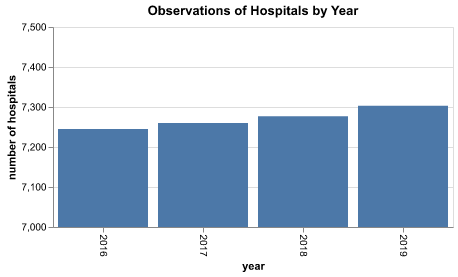
\includegraphics{chartQ1_3.png}

}

\caption{Chart Q1.3}

\end{figure}%

\paragraph{4. (Partner 1) Each hospital is identified by its CMS
certification number. Plot the number of unique hospitals in your
dataset per year. Compare this to your plot in the previous step. What
does this tell you about the structure of the
data?}\label{partner-1-each-hospital-is-identified-by-its-cms-certification-number.-plot-the-number-of-unique-hospitals-in-your-dataset-per-year.-compare-this-to-your-plot-in-the-previous-step.-what-does-this-tell-you-about-the-structure-of-the-data}

\begin{verbatim}
a.plot unique hospitals
\end{verbatim}

\begin{Shaded}
\begin{Highlighting}[]
\CommentTok{\#\#\# plot}
\NormalTok{df1\_4 }\OperatorTok{=}\NormalTok{ df.groupby(}\StringTok{\textquotesingle{}year\textquotesingle{}}\NormalTok{)[}\StringTok{\textquotesingle{}PRVDR\_NUM\textquotesingle{}}\NormalTok{].nunique().reset\_index()}

\NormalTok{chartQ1\_4 }\OperatorTok{=}\NormalTok{ alt.Chart(df1\_4).mark\_bar().encode(}
\NormalTok{    x}\OperatorTok{=}\NormalTok{ alt.X(}\StringTok{\textquotesingle{}year:O\textquotesingle{}}\NormalTok{, axis}\OperatorTok{=}\NormalTok{alt.Axis(labelAngle}\OperatorTok{=}\DecValTok{90}\NormalTok{)),}
\NormalTok{    y}\OperatorTok{=}\NormalTok{ alt.Y(}\StringTok{\textquotesingle{}PRVDR\_NUM:Q\textquotesingle{}}\NormalTok{, title}\OperatorTok{=}\StringTok{\textquotesingle{}number of unique hospitals\textquotesingle{}}\NormalTok{, scale}\OperatorTok{=}\NormalTok{alt.Scale(domain}\OperatorTok{=}\NormalTok{[}\DecValTok{7000}\NormalTok{, }\DecValTok{7500}\NormalTok{], clamp}\OperatorTok{=}\VariableTok{True}\NormalTok{))}
\NormalTok{).properties(}
\NormalTok{    width}\OperatorTok{=}\DecValTok{400}\NormalTok{, }
\NormalTok{    height}\OperatorTok{=}\DecValTok{200}\NormalTok{, }
\NormalTok{    title}\OperatorTok{=}\StringTok{\textquotesingle{}Unique Hospitals by Year\textquotesingle{}}  
\NormalTok{)}
\NormalTok{chartQ1\_4.save(}\StringTok{"chartQ1\_4.png"}\NormalTok{)}
\NormalTok{chartQ1\_4}
\end{Highlighting}
\end{Shaded}

\begin{verbatim}
alt.Chart(...)
\end{verbatim}

\begin{figure}[H]

{\centering 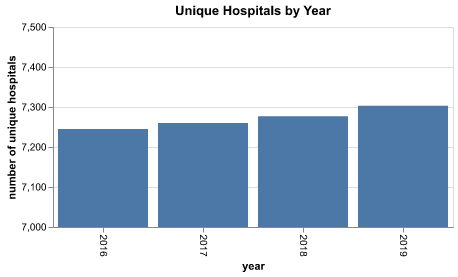
\includegraphics{chartQ1_4.png}

}

\caption{Chart Q1.4}

\end{figure}%

\begin{verbatim}
b.compare to previous step, what does this tell about data structure:
\end{verbatim}

The plots are identical. Which means each hospital is a unique
observation, tallied each year.

\subsection{Identify hospital closures in POS file (15 pts)
(*)}\label{identify-hospital-closures-in-pos-file-15-pts}

We will now use the 2016-2019 files to identify hospital closures
nationally. A hospital issuspected to have closed if its Termination
Code in the POS file lists them as an ``Active Provider'' in 2016 and
then they are either not active or do not appear in the data at all in a
subsequent year.

\paragraph{1. (Partner 2) Use this definition to create a list of all
hospitals that were active in 2016 that were suspected to have closed by
2019. Record the facility name and zip of each hospital as well as the
year of suspected closure (when they become terminated or disappear from
the data). How many hospitals are there that fit this
definition?}\label{partner-2-use-this-definition-to-create-a-list-of-all-hospitals-that-were-active-in-2016-that-were-suspected-to-have-closed-by-2019.-record-the-facility-name-and-zip-of-each-hospital-as-well-as-the-year-of-suspected-closure-when-they-become-terminated-or-disappear-from-the-data.-how-many-hospitals-are-there-that-fit-this-definition}

\paragraph{2. (Partner 2) Sort this list of hospitals by name and report
the names and year of suspected closure for the first 10
rows.}\label{partner-2-sort-this-list-of-hospitals-by-name-and-report-the-names-and-year-of-suspected-closure-for-the-first-10-rows.}

\paragraph{3. (Partner 2) However, not all suspected hospital closures
are true closures. For example, in the case of a merger, a CMS
certification number will be appear to be ``terminated,'' but then the
hospital re-appear under a similar name/address with a new CMS certifi
cation number in the next year. As a first pass to address this, remove
any suspected hospital closures that are in zip codes where the number
of active hospitals does not decrease in the year after the suspected
closure.}\label{partner-2-however-not-all-suspected-hospital-closures-are-true-closures.-for-example-in-the-case-of-a-merger-a-cms-certification-number-will-be-appear-to-be-terminated-but-then-the-hospital-re-appear-under-a-similar-nameaddress-with-a-new-cms-certifi-cation-number-in-the-next-year.-as-a-first-pass-to-address-this-remove-any-suspected-hospital-closures-that-are-in-zip-codes-where-the-number-of-active-hospitals-does-not-decrease-in-the-year-after-the-suspected-closure.}

\begin{verbatim}
a. Among the suspected closures, how many hospitals fit this definition of potentially being a merger/acquisition?

b. After correcting for this, how many hospitals do you have left?

c. Sort this list of corrected hospital closures by name and report the first 10 rows.
\end{verbatim}

\subsection{Download Census zip code shapefile (10
pt)}\label{download-census-zip-code-shapefile-10-pt}

Navigate to the Census shapefiles (link), select
``gz\_2010\_us\_860\_00\_500k.zip'' and download the resulting
shapefile. Note: If you have difficulty downloading or working with the
file because the size is too large for your computer, reach out to the
instruction team on Ed so that we can give them a smaller initial
shapefile to work with.

\paragraph{1. (Partner 1) This is non-tabular data. 1a. What are the
five file types and what type of information is in each file? 1b. It
will be useful going forward to have a sense going forward of which
files are big versus small. After unzipping, how big is each of the
datasets?}\label{partner-1-this-is-non-tabular-data.-1a.-what-are-the-five-file-types-and-what-type-of-information-is-in-each-file-1b.-it-will-be-useful-going-forward-to-have-a-sense-going-forward-of-which-files-are-big-versus-small.-after-unzipping-how-big-is-each-of-the-datasets}

\begin{verbatim}
a.

b. 
\end{verbatim}

\paragraph{2. (Partner 1) Load the zip code shapefile and restrict to
Texas zip codes. (Hint: you can identify which state a zip code is in
using the first 2-3 numbers in the zip code (Wikipedia link). Then
calculate the number of hospitals per zip code in 2016 based on the
cleaned POS file from the previous step. Plot a choropleth of the number
of hospitals by zip code in
Texas.}\label{partner-1-load-the-zip-code-shapefile-and-restrict-to-texas-zip-codes.-hint-you-can-identify-which-state-a-zip-code-is-in-using-the-first-2-3-numbers-in-the-zip-code-wikipedia-link.-then-calculate-the-number-of-hospitals-per-zip-code-in-2016-based-on-the-cleaned-pos-file-from-the-previous-step.-plot-a-choropleth-of-the-number-of-hospitals-by-zip-code-in-texas.}

\subsection{Calculate zip code's distance to the nearest hospital (20
pts)
(*)}\label{calculate-zip-codes-distance-to-the-nearest-hospital-20-pts}

\paragraph{1. (Partner 2) Create a GeoDataFrame for the centroid of each
zip code nationally: zips\_all\_centroids. What are the dimensions of
the resulting GeoDataFrame and what do each of the columns
mean?}\label{partner-2-create-a-geodataframe-for-the-centroid-of-each-zip-code-nationally-zips_all_centroids.-what-are-the-dimensions-of-the-resulting-geodataframe-and-what-do-each-of-the-columns-mean}

\paragraph{2. (Partner 2) Create two GeoDataFrames as subsets of
zips\_all\_centroids. First, create all zip codes in Texas:
zips\_texas\_centroids. Then, create all zip codes in Texas or a
bordering state: zips\_texas\_borderstates\_centroids, using the zip
code prefixes to make these subsets. How many unique zip codes are in
each of these
subsets?}\label{partner-2-create-two-geodataframes-as-subsets-of-zips_all_centroids.-first-create-all-zip-codes-in-texas-zips_texas_centroids.-then-create-all-zip-codes-in-texas-or-a-bordering-state-zips_texas_borderstates_centroids-using-the-zip-code-prefixes-to-make-these-subsets.-how-many-unique-zip-codes-are-in-each-of-these-subsets}

\paragraph{3.(Partner 2) Then create a subset of
zips\_texas\_borderstates\_centroids that contains only the zip codes
with at least 1 hospital in 2016. Call the resulting GeoDataFrame
zips\_withhospital\_centroids What kind of merge did you decide to do,
and what variable are you merging
on?}\label{partner-2-then-create-a-subset-of-zips_texas_borderstates_centroids-that-contains-only-the-zip-codes-with-at-least-1-hospital-in-2016.-call-the-resulting-geodataframe-zips_withhospital_centroids-what-kind-of-merge-did-you-decide-to-do-and-what-variable-are-you-merging-on}

\paragraph{4. (Partner 2) For each zip code in zips\_texas\_centroids,
calculate the distance to the nearest zip code with at least one
hospital in
zips\_withhospital\_centroids.}\label{partner-2-for-each-zip-code-in-zips_texas_centroids-calculate-the-distance-to-the-nearest-zip-code-with-at-least-one-hospital-in-zips_withhospital_centroids.}

\begin{verbatim}
a. This is a computationally-intensive join. Before attempting to do the entire join, subset to 10 zip codes in zips_texas_centroids and try the join. How long did it take? Approximately how long do you estimate the entire procedure will take?

b. Now try doing the full calculation and time how long it takes. How close is it to your estimation?

c. Look into the .prj file and report which unit it is in. Convert the given unit to miles, using an appropriate conversion you find online (estimates are okay).
\end{verbatim}

\paragraph{5.(Partner 2) Calculate the average distance to the nearest
hospital for each zip code in
Texas.}\label{partner-2-calculate-the-average-distance-to-the-nearest-hospital-for-each-zip-code-in-texas.}

\begin{verbatim}
a. What unit is this in

b. Report the average distance in miles. Does this value make sense?

c. Map the value for each zip code
\end{verbatim}

\subsection{Effects of closures on access in Texas (15
pts)}\label{effects-of-closures-on-access-in-texas-15-pts}

\paragraph{1. (Partner 1) Using the corrected hospital closures dataset
from the first section, create a list of directly affected zip codes in
Texas-- that is, those with at least one closure in 2016-2019. Display a
table of the number of zip codes vs.~the number of closures they
experienced.}\label{partner-1-using-the-corrected-hospital-closures-dataset-from-the-first-section-create-a-list-of-directly-affected-zip-codes-in-texas-that-is-those-with-at-least-one-closure-in-2016-2019.-display-a-table-of-the-number-of-zip-codes-vs.-the-number-of-closures-they-experienced.}

\paragraph{2.(Partner 1) Plot a choropleth of which Texas zip codes were
directly affected by a closure in 2016-2019-- there was at least one
closure within the zip code. How many directly affected zip codes are
there in
Texas?}\label{partner-1-plot-a-choropleth-of-which-texas-zip-codes-were-directly-affected-by-a-closure-in-2016-2019-there-was-at-least-one-closure-within-the-zip-code.-how-many-directly-affected-zip-codes-are-there-in-texas}

\paragraph{3. (Partner 1) Then identify all the indirectly affected zip
codes: Texas zip codes within a 10-mile radius of the directly affected
zip codes. To do so, first create a GeoDataFrame of the directly
affected zip codes. Then create a 10-mile buffer around them. Then, do a
spatial join with the overall Texas zip code shapefile. How many
indirectly affected zip codes are there in
Texas?}\label{partner-1-then-identify-all-the-indirectly-affected-zip-codes-texas-zip-codes-within-a-10-mile-radius-of-the-directly-affected-zip-codes.-to-do-so-first-create-a-geodataframe-of-the-directly-affected-zip-codes.-then-create-a-10-mile-buffer-around-them.-then-do-a-spatial-join-with-the-overall-texas-zip-code-shapefile.-how-many-indirectly-affected-zip-codes-are-there-in-texas}

\paragraph{4.(Partner 1) Make a choropleth plot of the Texas zip codes
with a different color for each of the 3 categories: directly affected
by a closure, within 10 miles of closure but not directly affected, or
not
affected.}\label{partner-1-make-a-choropleth-plot-of-the-texas-zip-codes-with-a-different-color-for-each-of-the-3-categories-directly-affected-by-a-closure-within-10-miles-of-closure-but-not-directly-affected-or-not-affected.}

\subsection{Reflecting on the exercise (10
pts)}\label{reflecting-on-the-exercise-10-pts}

\paragraph{(Partner 1) The ``first-pass'' method we're using to address
incorrectly identified closures in the data is imperfect. Can you think
of some potential issues that could arise still and ways to do a better
job at confirming hospital
closures?}\label{partner-1-the-first-pass-method-were-using-to-address-incorrectly-identified-closures-in-the-data-is-imperfect.-can-you-think-of-some-potential-issues-that-could-arise-still-and-ways-to-do-a-better-job-at-confirming-hospital-closures}

\paragraph{(Partner 2) Consider the way we are identifying zip codes
affected by closures. How well does this reflect changes in
zip-code-level access to hospitals? Can you think of some ways to
improve this
measure?}\label{partner-2-consider-the-way-we-are-identifying-zip-codes-affected-by-closures.-how-well-does-this-reflect-changes-in-zip-code-level-access-to-hospitals-can-you-think-of-some-ways-to-improve-this-measure}




\end{document}
